\section{Results}
    \subsection{Initial Data Exploration}
        During the initial data exploration, some of the features that were discussed earlier were gathered. Due to the fact that some features are quite complex to retrieve, the initial retrieval did not cover them all. During the later stages of this project, we would like to make all our features visual in some way or another; we found that this gives valuable insights regarding the structuring of the data we are dealing with.
        
        To actually make the data that was gathered more useful, some plots were made. 
        Figures \ref{fig:language-frequency-plot}, \ref{fig:star-distribution-plot}, \ref{fig:number-of-members-per-project-plot} and \ref{fig:number-of-commits-all-plot} are generated from the data that was gathered from the sample.
        An important observation is that almost all the data that was gathered is strongly right skewed. %this makes are life a pain.
        This implies that we might need to normalize it in the future, but that decision is yet to be made. 
        
	    \begin{figure}
	        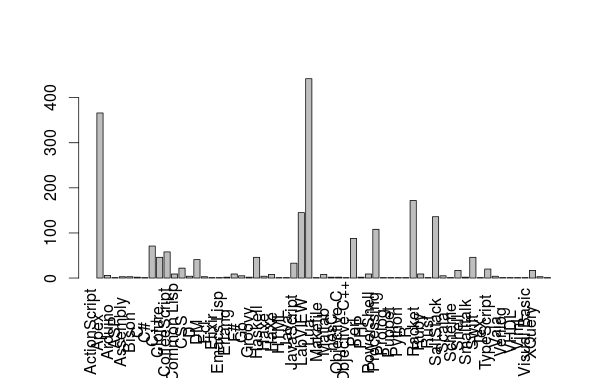
\includegraphics[width=250pt]{figures/language-frequency}
	        \caption{A histogram of the languages used in the projects}
	        \label{fig:language-frequency-plot}
	    \end{figure}

	    
	    \begin{figure}
	        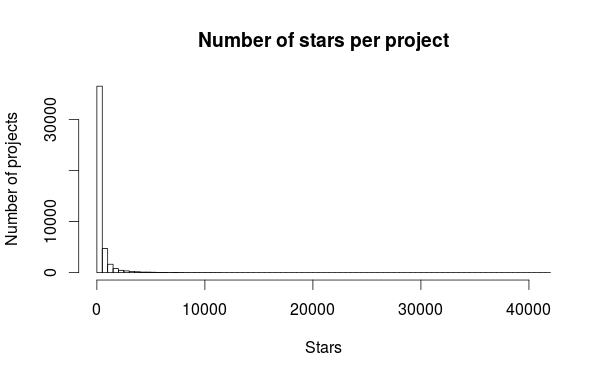
\includegraphics[width=250pt]{figures/star-distribution}
	        \caption{A histogram of the  number of stars per project}
	        \label{fig:star-distribution-plot}
	    \end{figure}
	    
	    \begin{figure}
	        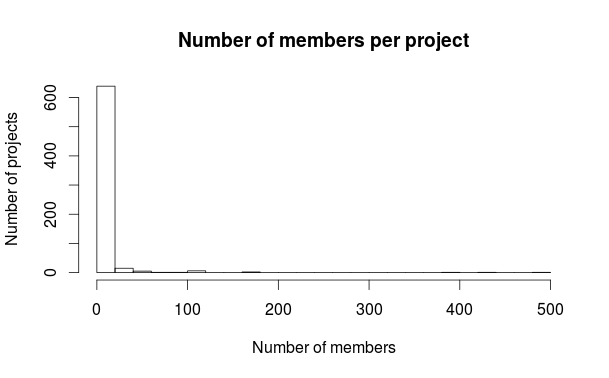
\includegraphics[width=250pt]{figures/number-of-members-per-project}
	        \caption{A histogram of the number of members per project}
	        \label{fig:number-of-members-per-project-plot}
	    \end{figure}
	    \begin{figure}
	        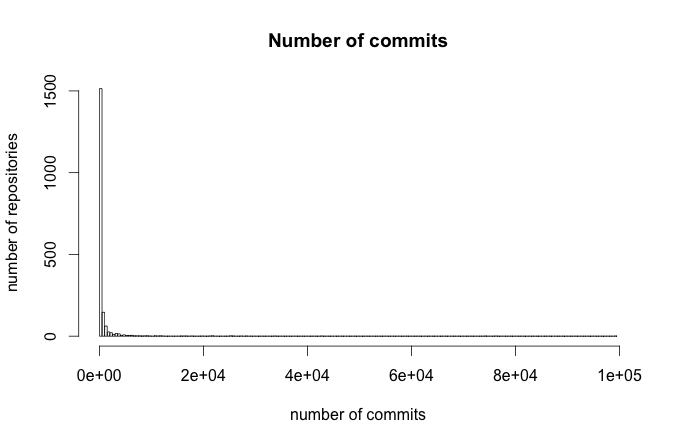
\includegraphics[width=250pt]{figures/number-of-commits-all}
	        \caption{A histogram of the number of commits per project}
	        \label{fig:number-of-commits-all-plot}
	    \end{figure}

    
    \subsection{Testing the model}
        \todo{Will be added later on, same for threats to validity}
